\section{Forward kinematics}
\subsection{Workspace}
\textbf{Kinematics} is the science of motion that treats motion without regard to the forces which cause it. One studies position, velocity, acceleration, and all higher order derivatives of position variables.

The existence or nonexistence of a kinematic solution defines the \textbf{workspace} of a given manipulator. If a solution doesn't exist, this means that the desired position/orientation lies outside of the manipulator's workspace. In other words, the workspace consists of all points that are reachable by the end-effector.

\subsubsection{Configuration}

The \textbf{configuration} of a moving object is a specification of the position of \textbf{every} point on the object. 

The \textbf{dimension of a config space} is the minimum number of parameters needed to specify the configuration of the object completely (also called the number of degrees of freedom of a moving object).

\subsubsection{Degrees of freedom}
The number of \textbf{degrees of freedom} that a manipulator possesses is the number of independent position variables that would have to be specified in order to locate all parts of the mechanism. E.g., industrial robotic manipulators often have as many d.o.f. as their number of joints, since each joint has one d.o.f. (and has 5 constraints).

\subsubsection{Right-hand-rule}
The signs of angles are determined by the direction of the fingers, when the thumb is pointing in the axis direction. Fingers also show the order of axis.

\begin{center}
	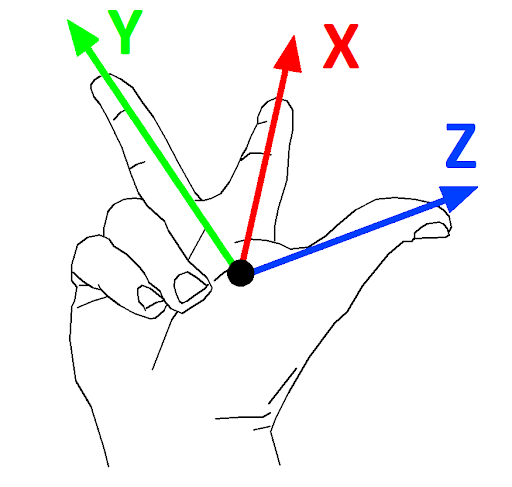
\includegraphics[width=5cm]{sections/imgs/2_right_hand_rule.png}
\end{center}

\subsection{Spatial descriptions}

We attach a coordinate system to a body and give a description of this coordinate system relative to the reference system. In Figure 2.2, system $B$ has been attached to the body, and its description relative to $A$ is given through its positions and orientation relative to $A$. 

\begin{center}
	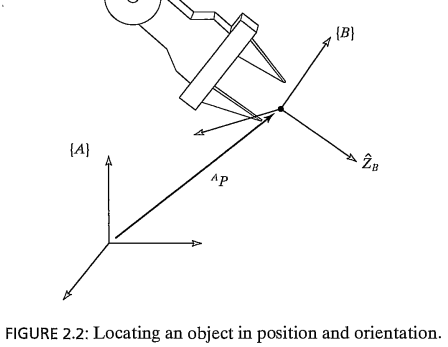
\includegraphics[width=9cm]{sections/imgs/2.png}
\end{center}

\subsubsection{Position}
\textbf{Description of a position:} Since many coordinate systems will be used, one has to define to which system a vector refers, e.g.,

\[^{A}\vect{p} = 
	\begin{bmatrix} p_x\\p_y\\p_z \end{bmatrix}, \] where $^{A}\vect{p}$ is a vector referring to coordinate system $A$.

\subsubsection{Orientation}
\textbf{Description of an orientation:} 
We stack three unit vectors (they specify the principal directions of the coord system) as columns, yielding the \textbf{rotation matrix:} 

\begin{center}
	$^{A}_{B}R = [^{A}\hat{X}_{B}\ ^{A}\hat{Y}_{B}\ ^{A}\hat{Z}_{B}] = 
	\begin{bmatrix} r_{11} & r_{12} & r_{13} \\ r_{21} & r_{22} & r_{23} \\ r_{31} & r_{32} & r_{33} \end{bmatrix} =\ ^{B}_{A} R^{-1} =\ ^{B}_{A} R^T$ \\
\end{center}
The rotation matrix has three constraints:
\begin{itemize}
	\item $|^{A}\hat{X}_{B}| = |^{A}\hat{Y}_{B}| = |^{A}\hat{Z}_{B}| = 1$
	\item $^{A}\hat{X}_{B} \cdot\ ^{A}\hat{Y}_{B} =\ ^{A}\hat{X}_{B} \cdot\ ^{A}\hat{Z}_{B} =\ ^{A}\hat{X}_{B} \cdot\ ^{A}\hat{Z}_{B} = 0$
	\item $\det{R} = 1$
\end{itemize}	
	
It describes the orientation of frame $B$ relative to frame $A$, i.e. it is used as a \textit{mapping} to \textbf{change the description of a vector from frame to frame}. Since we have unit magnitude and the vectors are orthogonal, the transposed matrix describes the orientation of system A written in B. These are orthonormal and length-preserving linear transformations. Also, rotation matrices preserve angles between vectors, i.e. $cos(\angle (\vect{p}, \vect{q})) = cos(\angle (R\vect{p}, R\vect{q}))$. The projection of a vector $\hat{X}_B$ in coord system $B$ into coord system $A$ is derived from the dot product with the principal directions of the coord frame of $A$, hence the graphic.
	
\begin{center}
	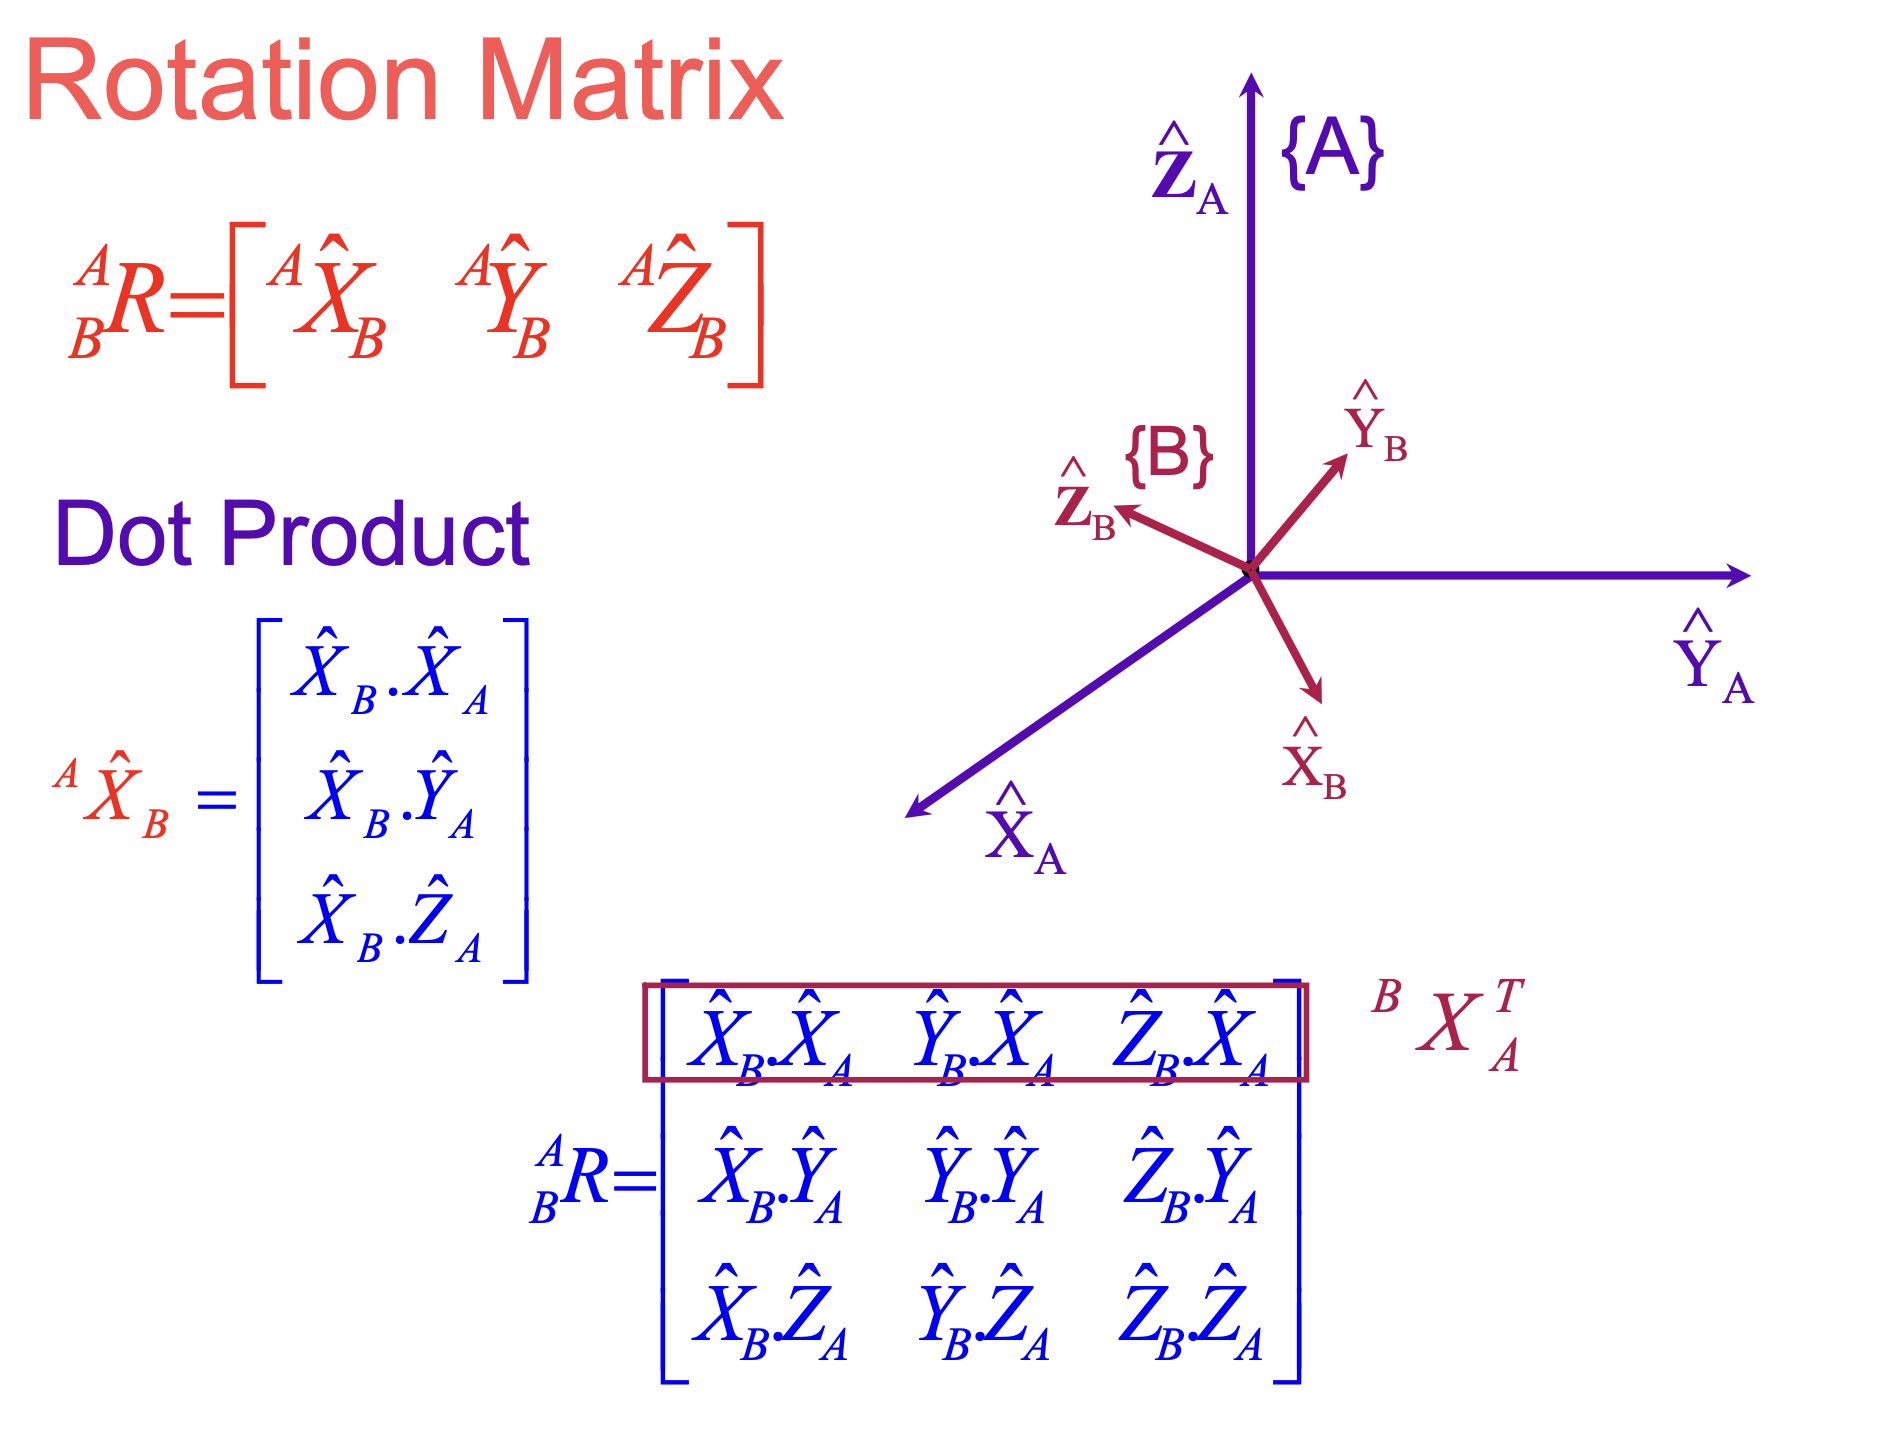
\includegraphics[width=9cm]{sections/imgs/2_rotation_matrix.png}
\end{center}

Besides mappings, another use case of rotation matrices is in the form of (rotational)\textit{operators} to move points within the same frame.

\subsubsection{Euler angles}
There is an issue when expressing orientations with a rotation matrix: When attempting to follow a trajectory in space by interpolating a current orientation from a start until a final orientation, the intermediary orientations are going to violate the constraints of the rotation matrix. Another possible description of a frame $B$ uses a \textit{three-angle-representation}. It works as follows: Frame $B$ coincides with a known frame $A$. Rotate $B$ first
\begin{itemize}
	\item about $ \hat{X}_{A} $ by an angle \(\gamma\), then about
	\item $ \hat{Y}_{A} $ by an angle \(\beta\), and finally about
	\item $ \hat{Z}_{A} $ by \(\alpha\).
\end{itemize}
If, each of the three rotations takes place about an axis in the fixed reference frame $A$, we call these angles \textit{X-Y-Z fixed angles}. An alternative representation uses angles that are relative to the previously changed coordinate frame, so-called \textbf{Euler angles}.

\begin{center}
	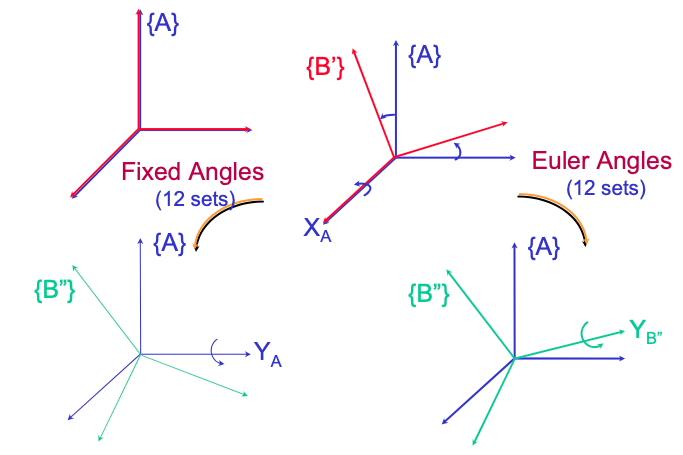
\includegraphics[width=10cm]{sections/imgs/2_fixed_relative_angles.png}
\end{center}

The next figure shows three subsequent rotations of a frame around the fixed axes $\hat X_A$, $\hat Y_A$ and $\hat Z_A$.

\begin{center}
	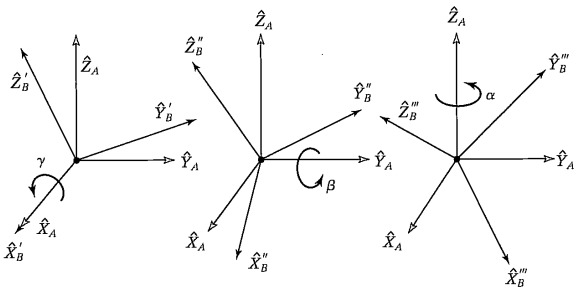
\includegraphics[width=10cm]{sections/imgs/9.png}
\end{center}

The combined rotation matrix is $^{A}_{B}R =\ ^{A}_{B'}R \cdot \ ^{B'}_{B''}R \cdot \ ^{B''}_{B}R$, which is cumbersome to compute. Instead, we define:

\begin{align*}
{ }_{B}^{A} R_{X Y Z}(\gamma, \beta, \alpha) &=R_{Z}(\alpha) R_{Y}(\beta) R_{X}(\gamma) \\
&=\left[\begin{array}{ccc}
\cos \alpha & -\sin \alpha & 0 \\ \sin \alpha & c \alpha & 0 \\ 0 & 0 & 1
\end{array}\right]\left[\begin{array}{ccc}
\cos \beta & 0 & \sin \beta \\ 0 & 1 & 0 \\ -\sin \beta & 0 & \cos \beta
\end{array}\right]\left[\begin{array}{ccc} 1 & 0 & 0 \\ 0 & \cos \gamma & -\sin \gamma \\
0 & \sin \gamma & \cos \gamma
\end{array}\right] \\
&= \left[\begin{array}{ccc}
\cos \alpha \cos \beta & \cos \alpha \sin \beta \sin \gamma-\sin \alpha \cos \gamma & \cos \alpha \sin \beta \cos \gamma+\sin \alpha \sin \gamma \\
\sin \alpha \cos \beta & \sin \alpha \sin \beta \sin \gamma+\cos \alpha \cos \gamma & \sin \alpha \sin \beta \cos \gamma-\cos \alpha \sin \gamma \\
-\sin \beta & \cos \beta \sin \gamma & \cos \beta \cos \gamma
\end{array}\right]
\end{align*}

When rotating a frame with Euler angles in the order of $Z$-$Y$-$X$, they produce the same combined rotation as $X$-$Y$-$Z$ fixed angles, i.e. $R_{Z^{\prime} Y^{\prime} X^{\prime}}(\alpha, \beta, \gamma)=R_{X Y Z}(\gamma, \beta, \alpha)$ for the same values of $(\alpha, \beta, \gamma)$. This next graphic shows the rotation using Euler angles:

\begin{center}
	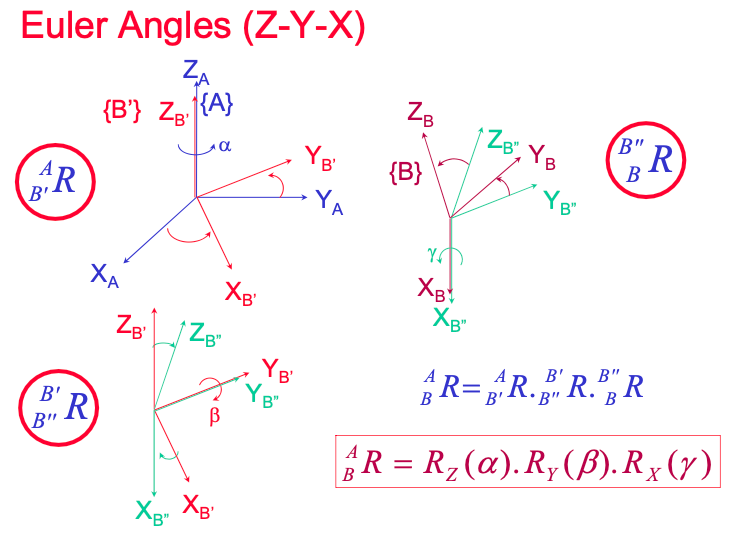
\includegraphics[width=10cm]{sections/imgs/2_euler_angles.png}
\end{center}

\textbf{Inverse problem:} Given $^{A}_{B}R$ find the $X$-$Y$-$Z$ fixed angles $(\alpha, \beta, \gamma)$. Let
\[{ }_{B}^A R_{X Y Z}(\gamma, \beta, \alpha)=\left[\begin{array}{lll}
r_{11} & r_{12} & r_{13} \\
r_{21} & r_{22} & r_{23} \\
r_{31} & r_{32} & r_{33}
\end{array}\right] \]

\begin{minipage}{0.4\textwidth}
Then:

\begin{align*}
&\beta=\operatorname{Atan} 2\left(-r_{31}, \sqrt{\left.r_{11}^{2}+r_{21}^{2}\right.}\right) \\
&\alpha=\operatorname{Atan} 2\left(r_{21} / \cos \beta, r_{11} / \cos \beta\right) \\
&\gamma=\operatorname{Atan} 2\left(r_{32} / \cos \beta, r_{33} / \cos \beta\right)
\end{align*}
	
\end{minipage}
\begin{minipage}{0.49\textwidth}
	\[ \operatorname{Atan} 2(a, b)= \begin{cases}\arctan \left(\frac{a}{b}\right) & \text { if } b>0 \\ \frac{\pi}{2} & \text { if } b=0, a>0 \\ \text { undefined } & \text { if } b=0, a=0 \\ -\frac{\pi}{2} & \text { if } b=0, a<0 \\ \arctan \left(\frac{a}{b}\right)+\pi & \text { if } b<0\end{cases} \]
\end{minipage}
\vspace{0.5cm}

 Note that for every parameter $(\alpha, \beta, \gamma)$ there are values which cause a singularity in this computation (e.g. for $\cos \beta = 0$).

\subsubsection{Unit quaternions (Euler parameters)}
Another representation of orientation is by means of four values called the \textbf{Euler parameters}. It can be shown that every rotation can be expressed as one rotation of $\theta$ around a single axis $K = [k_x\ k_y\ k_z]^T$. This is also known as the \textit{equivalent angle-axis representation}. 

\begin{center}
	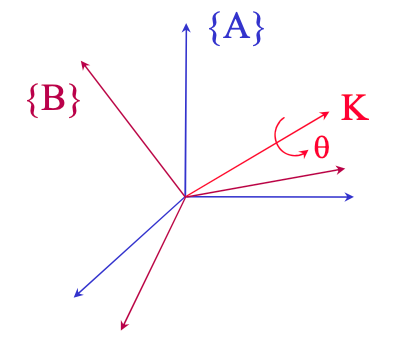
\includegraphics[width=4cm]{sections/imgs/2_equivalent_angle_axis.png}
\end{center}

The Euler parameters are given by

\[ (\varepsilon_1 , \varepsilon_2 , \varepsilon_3 , \varepsilon_4) = ( k_{x} \sin \frac{\theta}{2}, k_{y} \sin \frac{\theta}{2}, k_{z} \sin \frac{\theta}{2}, \cos \frac{\theta}{2})  \]

and 
\[ \epsilon_{1}^{2}+\epsilon_{2}^{2}+\epsilon_{3}^{2}+\epsilon_{4}^{2}=1 \]

This $4 \times 1$ vector is known as a unit quaternion, the orientation it describes could be visualized as a point on a unit hypersphere in four-dimensional space. It turns out that the orientation representation through Euler parameters does not have a singularity.


\subsection{Spatial transformations}
\textit{Problem:} We know the definition of a vector with respect to some frame $B$ and we would like to express it with respect to another frame $A$, where the origins of the two frames are coincident. We can compute this, if we know a description of the orientation of $B$ relative to $A$. Then, \[^{A} P = {^{A}_{B}}R\ {^{B}}P \] computes what a \textbf{vector that is expressed in coordinate system B ``looks like'' if observed from system A}.

\begin{center}
	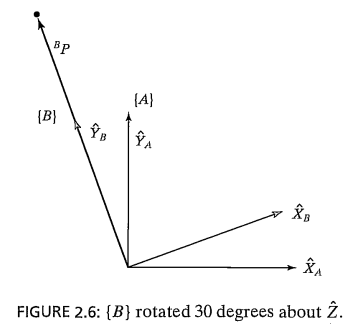
\includegraphics[width=5cm]{sections/imgs/4.png} 
	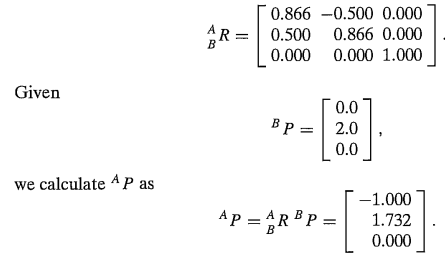
\includegraphics[width=7cm]{sections/imgs/5.png}	
\end{center}

Now, the \textbf{general case}, where the systems don't have the same origin, but B is shifted by $P_{BORG}$ from the origin (or $^{A}P_{BORG}$ when expressed in $A$):

$$^{A}P =\ ^{A}_{B}R\ ^{B}P + \ ^{A}P_{BORG}\ $$ 

\begin{center}
	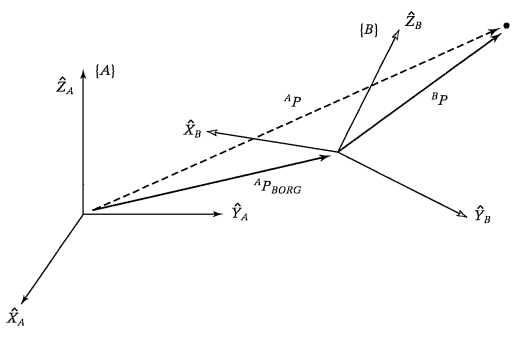
\includegraphics[width=6cm]{sections/imgs/6.png}
\end{center}

Computing a position of a point connected by multiple subsequent links of a manipulator with individual coordinate frames, involves the multiplication of sums given by the general transform equation. This is because \textit{rotation} and \textit{translation} are both needed to propagate from one frame to another. To simplify this calculation, a \textbf{homogeneous transform} combines rotation and translation into a matrix $_{B}^{A}T$, such that: ${}^{A}P={}_{B}^{A}T\ ^{B}P$. Therefore, the homogeneous transform is a \textit{general operator}.

\begin{center}
	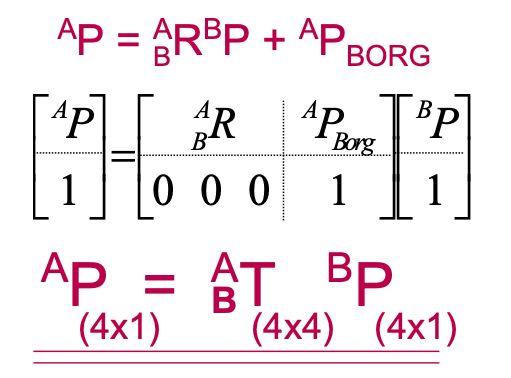
\includegraphics[width=4cm]{sections/imgs/2_homogeneous_transform.png}
\end{center}

Due to the generality of the homogeneous transform, it can be interpreted in different ways: 1.) as a description of a frame $\{B\}=\{_{B}^{A}R \ \ ^{A}P_{BORG}\}$; 2.) as a mapping of a point in frame $B$ to frame $A$; 3.) as an operator to rotate and translate a point in the same frame. This is an example for the second case:

\begin{center}
	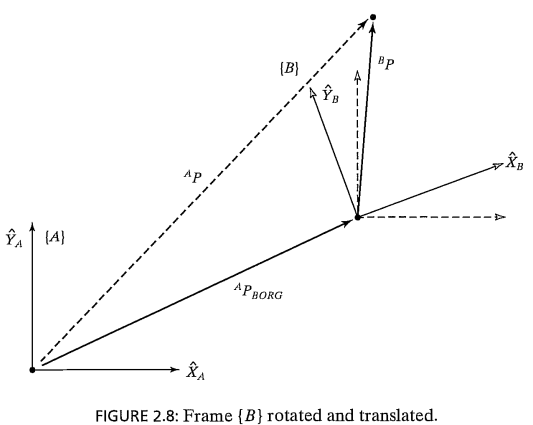
\includegraphics[width=6cm]{sections/imgs/7.png}
	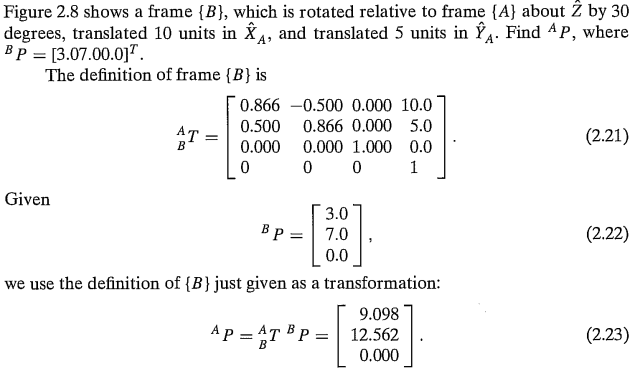
\includegraphics[width=8cm]{sections/imgs/8.png}
\end{center}
 
Inverse of the homogeneous transform:

\begin{center}
	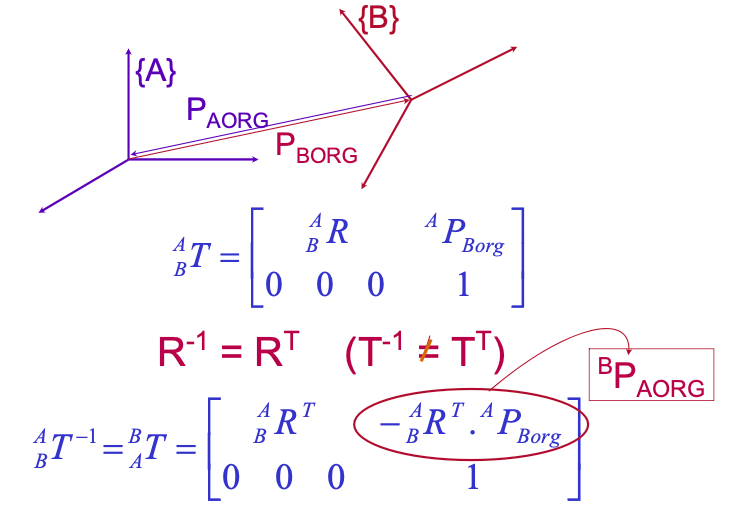
\includegraphics[width=7cm]{sections/imgs/2_inverse_transform.png}
\end{center}

Compound transformation:

\begin{center}
	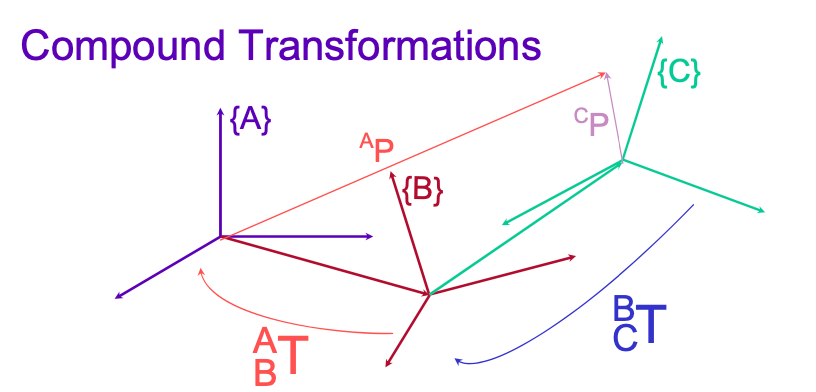
\includegraphics[width=7cm]{sections/imgs/2_compound_transformation_1.png}
	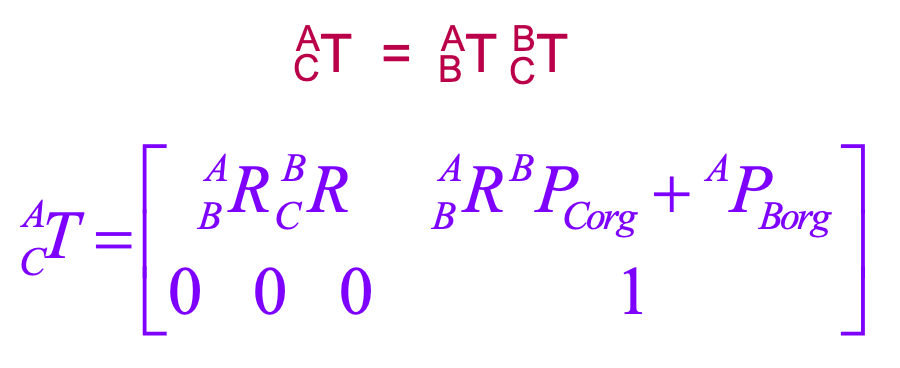
\includegraphics[width=6cm]{sections/imgs/2_compound_transformation_2.png}
\end{center}

Transform equation: ${}_{B}^{A}T \ {}_{C}^{B}T \ {}_{D}^{C}T \ {}_{A}^{D}T= I$.

\subsection{Forward kinematics}
Forward kinematics solves the static geometrical problem of computing the position and the orientation of the end-effector of the manipulator. Specifically, given a \textbf{set of joint angles}, the forward kinematic problem is to compute the position and orientation of the tool frame relative to the base frame.

\subsubsection{Denavit-Hartenberg Convention}
The homogeneous transform between consecutive frames of links is represented via only 4 D-H-parameters (x-rot, x-trans, z-trans, z-rot). In general, 6 parameters are needed to represent an arbitrary rigid body transformation! Thus, a restriction of it is, that it \textbf{cannot represent a rotation around the $y$-axis and that the $y$- and $z$-position are coupled}.

Procedure for deriving the D-H-parameters:

\begin{center}
	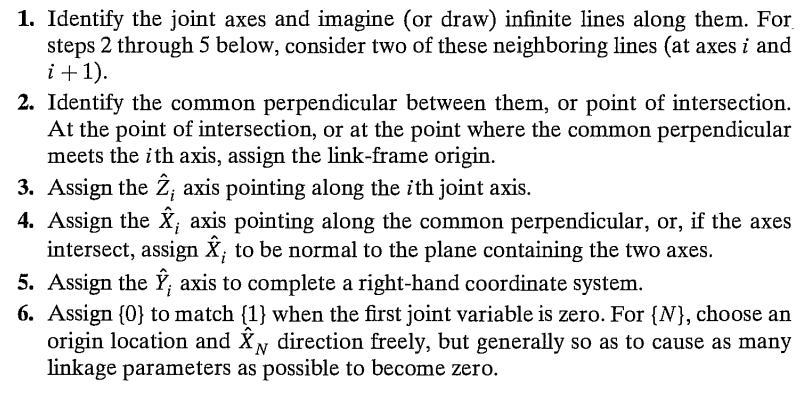
\includegraphics[width=13cm]{sections/imgs/10.png}\\
	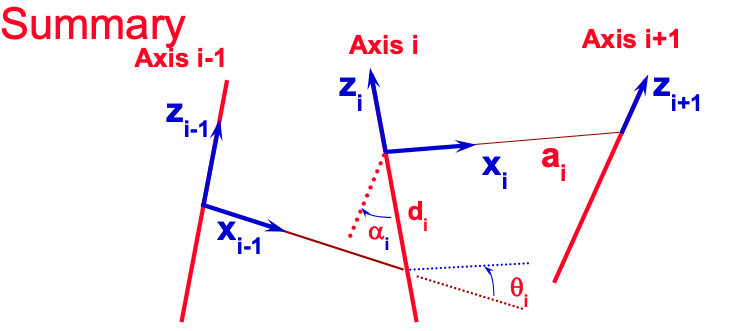
\includegraphics[width=7cm]{sections/imgs/2_dh_params.png}
	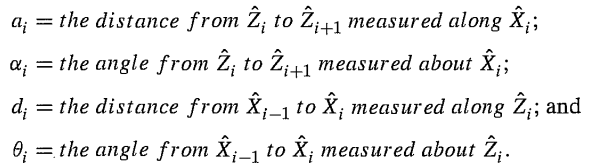
\includegraphics[width=9cm]{sections/imgs/11.png}
\end{center}

Among the four D-H-parameters are three fixed link parameters and one joint variable, which is $\theta_i$ for a revolute joint or $d_i$ for a prismatic joint. The D-H-parameters are plugged into homogenous transformation matrices, which represent the single transformations between the frames of subsequent links. Then, we can propagate through all homogeneous transformations to calculate the position and orientation of the end-effector. Hereafter, the above described procedure is detailed further:\\

\begin{figure*}[h]
	\centering
	\subfloat[Identify the joint axes; consider axes $i$ and $i-1$. By convention, a joint axis points \textbf{in the direction of the rotation/ movement} for revolute/ prismatic joints.]{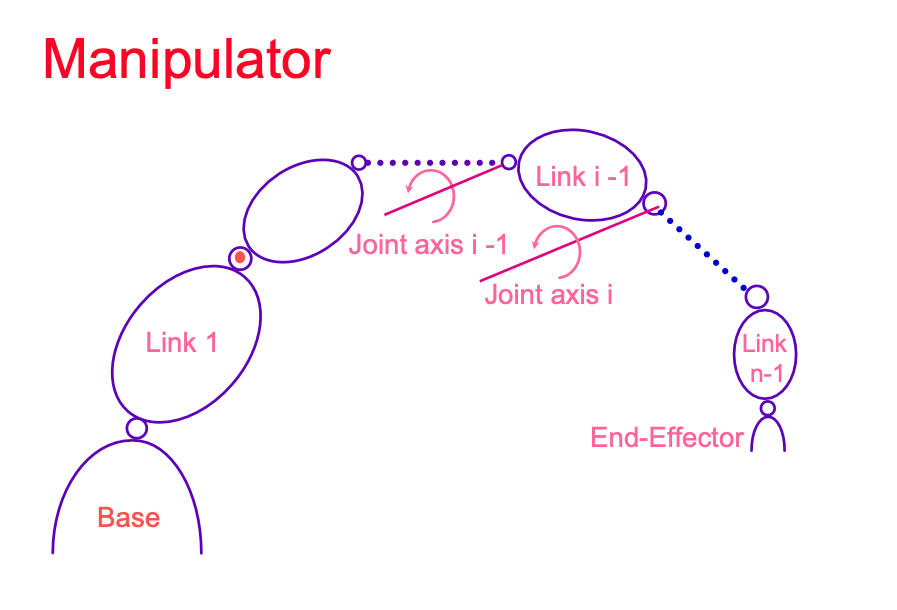
\includegraphics[width=.45\textwidth]{sections/imgs/2_dh_1.png}}
	\hfill
	\subfloat[Identify the common perpendicular. If the axes intersect, the common perpendicular is a normal through the plane they span and the direction of $\alpha_i$ is determined by the direction of this normal. \textbf{$a_i$ and $\alpha_i$ describe the $i$th link}. (``We rotate axis $i-1$ around the normal about $\alpha$ so that it coincides with axis $i$. This aligns the $Z$-axes.'')]{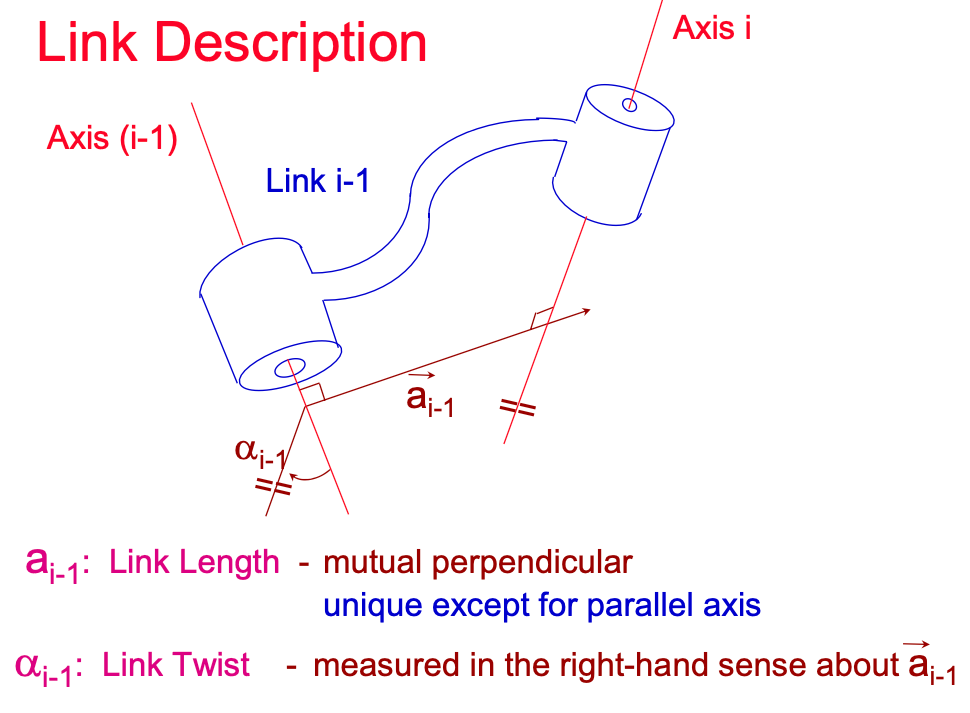
\includegraphics[width=.45\textwidth]{sections/imgs/2_dh_2.png}}\\
\end{figure*}

\begin{figure*}[h]
	\ContinuedFloat
	\centering
	\subfloat[\textbf{$d_i$ and $\theta_i$ describe the $i-1$th link connection}. If the axes of link $i-1$ and link $i$ are parallel, the origin of a coordinate frame $\{i-1\} $ should be attached, such that $d_i=0$. (``$\theta_i$ aligns the $X$-axes by rotation around $Z_i$.'')]{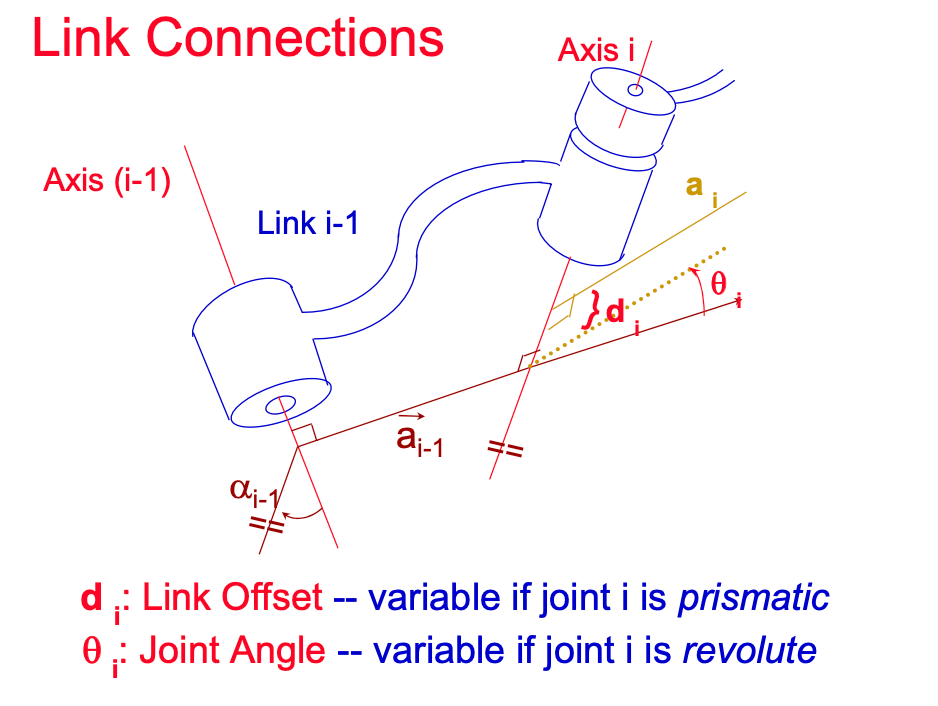
\includegraphics[width=.45\textwidth]{sections/imgs/2_dh_3.png}}
	\hfill
	\subfloat[Attach $i$th frame, such that $\hat Z_i$ is in the direction of the $i$th joint axis and $\hat X_i$ points along the common perpendicular (if $\hat Z_{i-1}$ and $\hat Z_i$ intersect, choose $\hat X_{i-1}$, such that $\alpha_{i-1}>0$). $\hat Y_i$ completes the right-hand frame.]{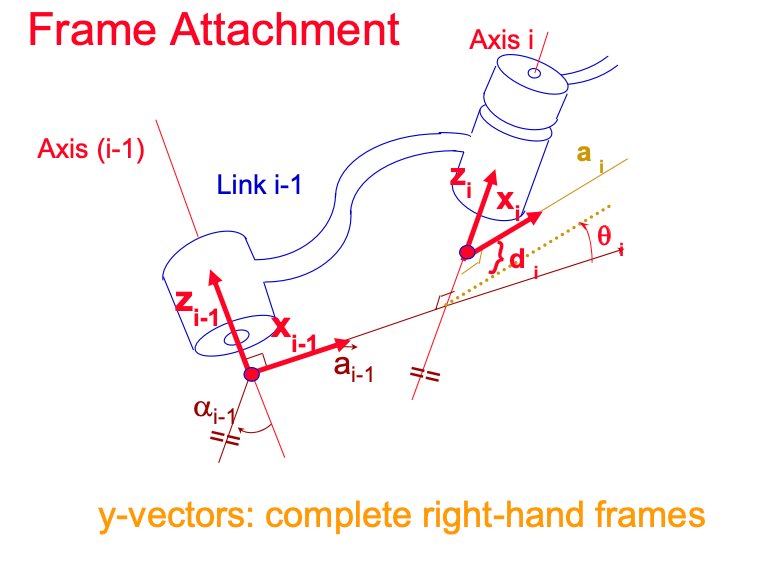
\includegraphics[width=.45\textwidth]{sections/imgs/2_dh_4.png}}\\
\end{figure*}

\begin{figure}[h]
	\ContinuedFloat 
	\centering
	\subfloat[$a_i$ and $\alpha_i$ depend on joint axes $i$ and $i+1$. Thus, select axes $0$ and $n+1$, such that $a_0=a_n=0$ and $\alpha_0=\alpha_n=0$ (by making axis $0$ coincident with axis $1$ and axis $n+1$ coincident with axis $n$). This simplifies the forward kinematics.]{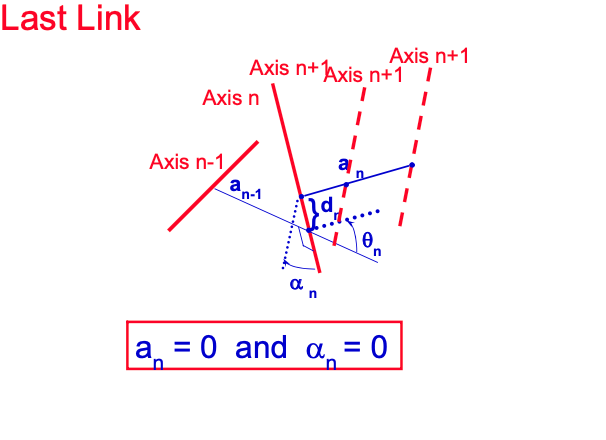
\includegraphics[width=.45\textwidth]{sections/imgs/2_dh_5.png}}
	\hfill
	\subfloat[$\theta_i$ and $d_i$ depend on joint axes $i$ and $i-1$. Again, select axes $0$ and $n+1$, such that depending on the joint type $a_0$ or $\theta_0=0$ and $a_n$ or $\theta_n=0$ (by coinciding axes and moving the intersection point that becomes the origin of the frame so that $d=0$ or orienting the axis so that $\theta=0$). ]{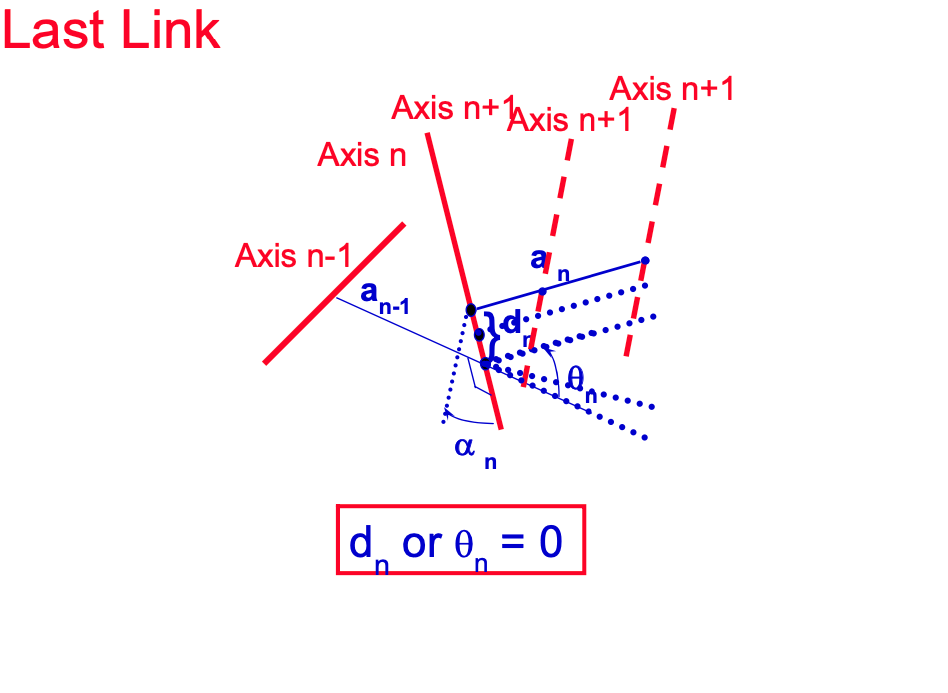
\includegraphics[width=.45\textwidth]{sections/imgs/2_dh_6.png}}
\end{figure}
 
\begin{figure}[h]
	\ContinuedFloat 
	\centering
	\subfloat[$\{0\}$ is assigned, such that is equals $\{1\}$ when the first joint variable is $0$.]{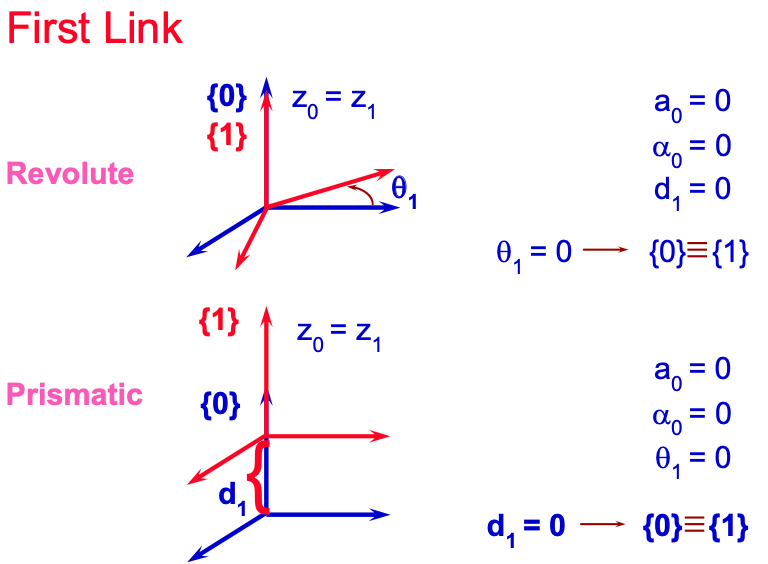
\includegraphics[width=.45\textwidth]{sections/imgs/2_dh_7.png}}
	\hfill
	\subfloat[Assign $\{N\}$, such that the most parameters are $0$.]{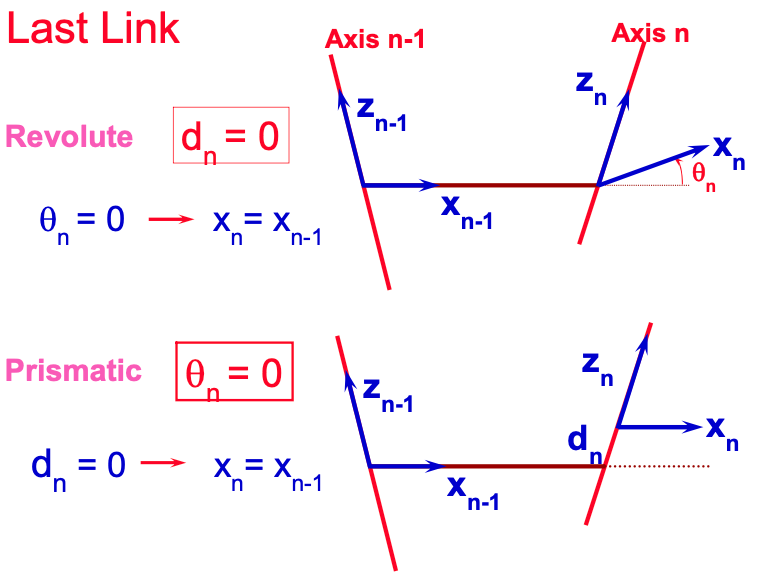
\includegraphics[width=.45\textwidth]{sections/imgs/2_dh_8.png}}
\end{figure}

\FloatBarrier

Then, the forward kinematics of a single link using the D-H-parameters derive as follows:

\begin{figure}[h]
	\centering
	\subfloat[To obtain $^{i-1}_{i}T$: Translate along $Z_{i}$ about $d_i$ ($\rightarrow \{P\} $), then rotate around $Z_i$ about $\theta_i$ ($\rightarrow \{Q\} $), then translate along $X_{i-1}$ about $a_{i-1}$ ($\rightarrow \{R\} $) and finally rotate around $X_i$ about $\alpha_i$ ($\rightarrow \{i-1\} $). This results in the homogeneous transform for a single link from $\{i\} $ to $\{i-1\} $ and also works in the other direction to compute the inverse homogeneous transform.]{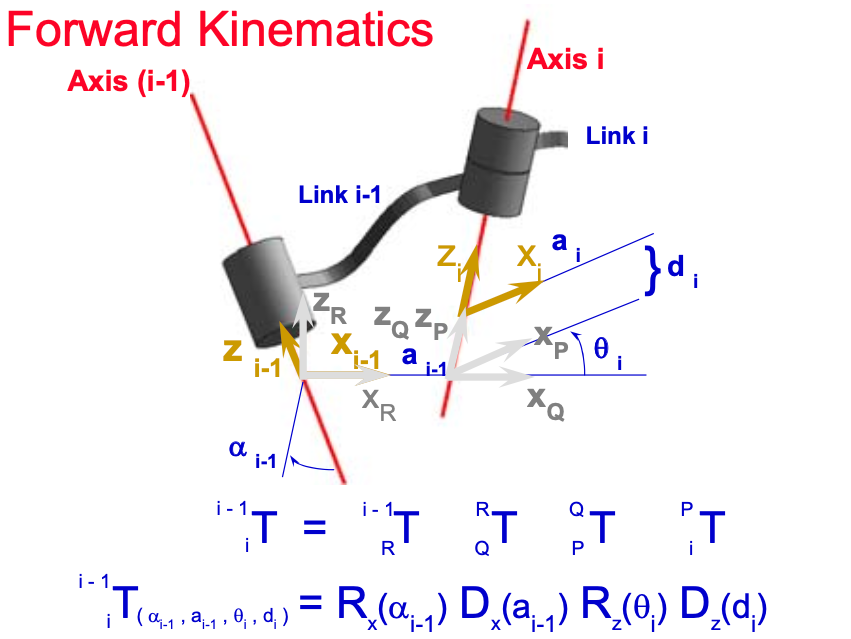
\includegraphics[width=.45\textwidth]{sections/imgs/2_dh_fkin_1.png}}
	\hfill
	\subfloat[The \textbf{homogeneous transformation from link $i$ to link $i-1$} (the formula in the slide should say $i$ instead of $1$).]{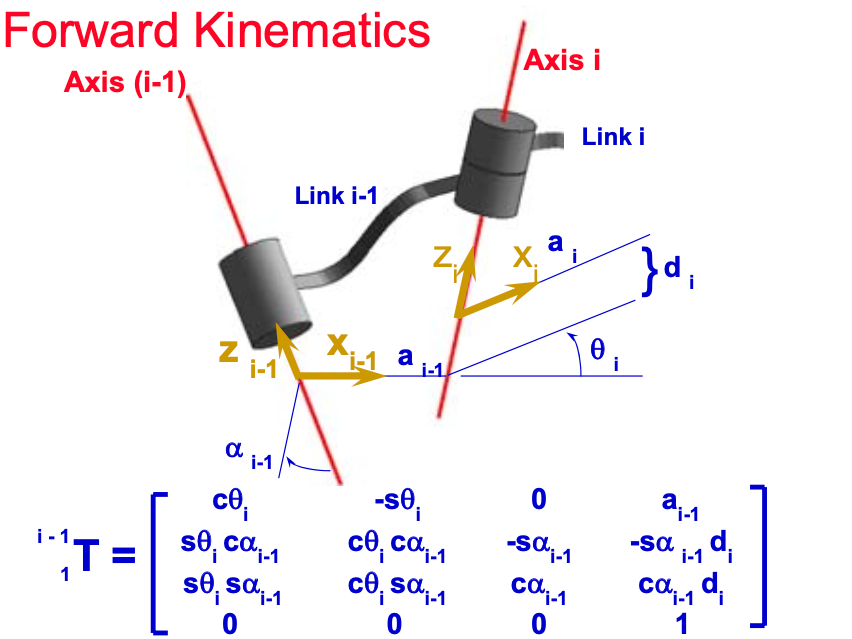
\includegraphics[width=.45\textwidth]{sections/imgs/2_dh_fkin_2.png}}\\
	\subfloat[The homogeneous transformation which transforms points from the frame of link $N$ to the frame of link $0$.]{
\includegraphics[width=.45\textwidth]{sections/imgs/2_dh_fkin_3.png}}
	
\end{figure}

Note, that the homogeneous transform ${}^{i-1}_iT$ cannot express arbitrary rigid body transformations, since no rotation about $\hat{Y}$ is possible.
A good, practical explanation of how to place the coordinate frames at each link, derive the D-H-parameters and compute the homogeneous transformations and forward kinematics is given in \href{https://youtu.be/u79KfNgP1Cc?t=1939}{this video} (based on an example).